% Options for packages loaded elsewhere
\PassOptionsToPackage{unicode}{hyperref}
\PassOptionsToPackage{hyphens}{url}
%
\documentclass[
  12pt,
]{article}
\title{Air Quality in Ukraine post Ukraine-Russia Dispute}
\usepackage{etoolbox}
\makeatletter
\providecommand{\subtitle}[1]{% add subtitle to \maketitle
  \apptocmd{\@title}{\par {\large #1 \par}}{}{}
}
\makeatother
\subtitle{Web address for GitHub repository}
\author{Shirley Fontanié, Rachel Gordon, and Julia Weinberg}
\date{}

\usepackage{amsmath,amssymb}
\usepackage{lmodern}
\usepackage{iftex}
\ifPDFTeX
  \usepackage[T1]{fontenc}
  \usepackage[utf8]{inputenc}
  \usepackage{textcomp} % provide euro and other symbols
\else % if luatex or xetex
  \usepackage{unicode-math}
  \defaultfontfeatures{Scale=MatchLowercase}
  \defaultfontfeatures[\rmfamily]{Ligatures=TeX,Scale=1}
  \setmainfont[]{Times New Roman}
\fi
% Use upquote if available, for straight quotes in verbatim environments
\IfFileExists{upquote.sty}{\usepackage{upquote}}{}
\IfFileExists{microtype.sty}{% use microtype if available
  \usepackage[]{microtype}
  \UseMicrotypeSet[protrusion]{basicmath} % disable protrusion for tt fonts
}{}
\makeatletter
\@ifundefined{KOMAClassName}{% if non-KOMA class
  \IfFileExists{parskip.sty}{%
    \usepackage{parskip}
  }{% else
    \setlength{\parindent}{0pt}
    \setlength{\parskip}{6pt plus 2pt minus 1pt}}
}{% if KOMA class
  \KOMAoptions{parskip=half}}
\makeatother
\usepackage{xcolor}
\IfFileExists{xurl.sty}{\usepackage{xurl}}{} % add URL line breaks if available
\IfFileExists{bookmark.sty}{\usepackage{bookmark}}{\usepackage{hyperref}}
\hypersetup{
  pdftitle={Air Quality in Ukraine post Ukraine-Russia Dispute},
  pdfauthor={Shirley Fontanié, Rachel Gordon, and Julia Weinberg},
  hidelinks,
  pdfcreator={LaTeX via pandoc}}
\urlstyle{same} % disable monospaced font for URLs
\usepackage[margin=2.54cm]{geometry}
\usepackage{longtable,booktabs,array}
\usepackage{calc} % for calculating minipage widths
% Correct order of tables after \paragraph or \subparagraph
\usepackage{etoolbox}
\makeatletter
\patchcmd\longtable{\par}{\if@noskipsec\mbox{}\fi\par}{}{}
\makeatother
% Allow footnotes in longtable head/foot
\IfFileExists{footnotehyper.sty}{\usepackage{footnotehyper}}{\usepackage{footnote}}
\makesavenoteenv{longtable}
\usepackage{graphicx}
\makeatletter
\def\maxwidth{\ifdim\Gin@nat@width>\linewidth\linewidth\else\Gin@nat@width\fi}
\def\maxheight{\ifdim\Gin@nat@height>\textheight\textheight\else\Gin@nat@height\fi}
\makeatother
% Scale images if necessary, so that they will not overflow the page
% margins by default, and it is still possible to overwrite the defaults
% using explicit options in \includegraphics[width, height, ...]{}
\setkeys{Gin}{width=\maxwidth,height=\maxheight,keepaspectratio}
% Set default figure placement to htbp
\makeatletter
\def\fps@figure{htbp}
\makeatother
\setlength{\emergencystretch}{3em} % prevent overfull lines
\providecommand{\tightlist}{%
  \setlength{\itemsep}{0pt}\setlength{\parskip}{0pt}}
\setcounter{secnumdepth}{5}
\ifLuaTeX
  \usepackage{selnolig}  % disable illegal ligatures
\fi

\begin{document}
\maketitle

\newpage
\tableofcontents 
\newpage
\listoftables 
\newpage
\listoffigures 
\newpage

\hypertarget{rationale-and-research-questions}{%
\section{Rationale and Research
Questions}\label{rationale-and-research-questions}}

\begin{quote}
During periods of war and geopolitical conflicts, environmental
pollution and degraded air quality is a common effect experienced by
nations subject to violent attacks. Specifically, the use of explosive
weapons can cause extensive damage to urban buildings and
infrastructure, resulting in hazardous dust, debris, and other air
particles that can have lasting health impacts on affected populations.
\end{quote}

\begin{quote}
On February 24, 2022 Russia invaded Ukraine due to geopolitical
conflicts between the two nations. Russia's invasion has consisted of
multiple missile attacks throughout Ukraine, causing extensive damage to
urban infrastructure, reducing buildings to rubble and creating
dangerous explosions that have enormous potential to raise air pollution
levels. Therefore, in this project, we examine two different Ukrainian
cities that have experienced attacks since Russia's invasion and explore
air quality levels of these cities both before and during the war.
\end{quote}

\begin{quote}
As the conflict has been ongoing throughout all of March 2022, we chose
to analyze air quality data from March 2022 as well as March 2021. We
chose to include data from the same month in 2021 to be able to compare
air quality levels during the war to the levels before to control for
weather and temperature variations that typically occur throughout
different months and seasons. Additionally, we were interested in
exploring air quality levels of two cities that are in different
geographic locations and have experienced at least one missile attack by
Russia during March 2022. For air quality indicators, we wanted to look
at both PM 2.5 and PM 10, as the levels of these particulate matters
increase from sources such as construction sites and fires and can have
lasting effects on human health. PM2.5 are very fine inhalable particles
that are 2.5 micrometers or smaller, whereas PM10 are less than 10.5
micrometers. Lastly, we wanted to look at two cities that differed in
economic activity and levels of industrial manufacturing, as industrial
manufacturing activities can have an effect on air quality levels.
\end{quote}

\newpage

\hypertarget{dataset-information}{%
\section{Dataset Information}\label{dataset-information}}

\begin{quote}
Data for this project was retrieved from the World Air Quality Indices'
Air Quality Historical Data Platform. The World Air Quality Index is a
non-profit started in 2007 that is working to increase transparency for
air quality data in order to improve pollution awareness. The World Air
Quality Index created the Air Quality Historical Data Platform in 2014
in order to provide information on how location-based air quality is
changing over time. Data in this report looks at PM10 and PM2.5 air
pollution. The World Air Quality Index provides ranges for air quality
health and the numbers are differentiated for PM2.5 and PM10. Table 1
provides the ranges for good, moderate, poor, and unhealthy air quality
levels. Historical data sets available through the World Air Quality
Index span a 36-month time frame, and data used in this report is from
2019-2022. The data was collected for two cities Dnipro and Lviv,
located in Eastern and Western Ukraine respectively. The air-quality
monitoring station in Lviv is called Steeldrum and the air-quality
monitoring station in Dnipro is called Vulytsya-Pavla Nirinberha, 4-6.
\end{quote}

\begin{quote}
Initially once accessing our first csv dataset (outlined in Table 1), we
processed the UkraineData by omitting missing values (the NA's) from the
PM2.5 and PM 10 values.\\
Then, we set the ``numeric'' class of the date column to a ``date''
class. Then, we wrangled the processed version of the Ukraine data and
created four subsets by city, month, and year. Each city, Dnipro and
Lviv, is being evaluated for air quality during the month of March and
in years 2021 and 2022. Now we have four new data sets; Dnipro 2021,
Dnipro 2022, Lviv 2021, and Lviv 2022, all showing PM2.5 and PM10 values
for days in March. We then binded the rows for both Dnipro 2021 and
Dnipro 2022, called FULL\_DNIPRO. We also binded rows for Lviv 2021 and
Lviv 2022, called FULL\_LVIV.\\
In our exploratory analysis, we wanted to look at mean, maximum,
minimum, and the standard deviation for PM2.5 and PM10 values in Dnipro
and Ukraine. We used the group\_by function to group by City, and the
summarize function to include mean, maximum, minimum, and standard
deviation of the PM values. Additionally, within the exploratory
analysis we binded FULL\_Dnipro and FULL\_LVIV in order to create a dot
plot showing the air quality ranges our data demonstrated. We then
plotted this data with ggplot using scale\_fill\_gradient2 to color-code
data by health-hazard level. Furthermore, we wanted to look at PM2.5 and
PM10 values comparing Dnipro and Lviv in solely March 2022 -- during the
time of the missile attacks. To do this analysis, we wrangled the Dnipro
2022 and Lviv 2022 to create a dataset with both cities, that includes
both PM values, for solely March 2022. The important difference is that
we are not looking at 2021 values in this dataset. Table 2 outlines all
of our working data sets and what they each contain.
\end{quote}

\newpage

\textbf{Table 1}

\begin{longtable}[]{@{}lll@{}}
\toprule
Data File Name & Column Name & Data Type \\
\midrule
\endhead
UkraineData & City & Factor (Dnipro and Lviv) \\
UkraineData & Date & Factor (later converted to date object) \\
UkraineData & pm25 & Integer (PM2.5 values) \\
UkraineData & pm10 & Integer (PM10 values) \\
\bottomrule
\end{longtable}

\textbf{Table 2}

\begin{longtable}[]{@{}ll@{}}
\toprule
Data File Name & Description \\
\midrule
\endhead
UkraineData & (Raw) Ukraine air quality data \\
Ukraine\_Processed & (Processed) Ukraine air quality data, w/o na's \\
Dnipro\_2021 & Dnipro PM2.5 + PM10, Mar 2021 \\
Dnipro\_2022 & Dnipro PM2.5+ PM10, Mar 2022 \\
Lviv\_2021 & Lviv PM 2.5 + PM10, Mar 2021 \\
Lviv\_2022 & Lviv PM 2.5 + PM10, Mar 2022 \\
FULL\_LVIV & Lviv\_2021 + Lviv\_2022 combined \\
FULL\_Dnipro & Dnipro\_2021 + Dnipro\_2022 combined \\
FULL\_Air\_quality & Dnipro\_2022 + Lviv\_2022 combined \\
Full-air\_quality\_21\_22 & FULL\_LVIV + FULL\_Dnipro combined \\
\bottomrule
\end{longtable}

\newpage

\hypertarget{exploratory-analysis}{%
\section{Exploratory Analysis}\label{exploratory-analysis}}

\begin{quote}
To begin our exploratory analysis of the air quality data, we created
dot plots to map out what range of our quality our data fell into
(Figures 1 \& 2). The data is color coded with green denoting good air
quality conditions, yellow is moderate conditions, and red is showing
air quality that is poor and likely hazardous to health. Attached is a
table showing a breakdown for air quality metrics (Table 3). This dot
plot was created to show the range in which our data falls in terms of
air quality health. Additionally, we determined the summary statistics
of the PM10 and PM2.5 (Table 4)
\end{quote}

\textbf{Table 3}

\begin{longtable}[]{@{}lll@{}}
\toprule
AQI Category & PM2.5 & PM10 \\
\midrule
\endhead
Good & 0 to 15.5 & 0 to 54 \\
Moderate & 15.5 to 35.5 & 54 to 150 \\
Poor & 35.5 to 150 & 150 to 250 \\
Unhealthy & 150+ & 250+ \\
\bottomrule
\end{longtable}

\begin{figure}
\centering
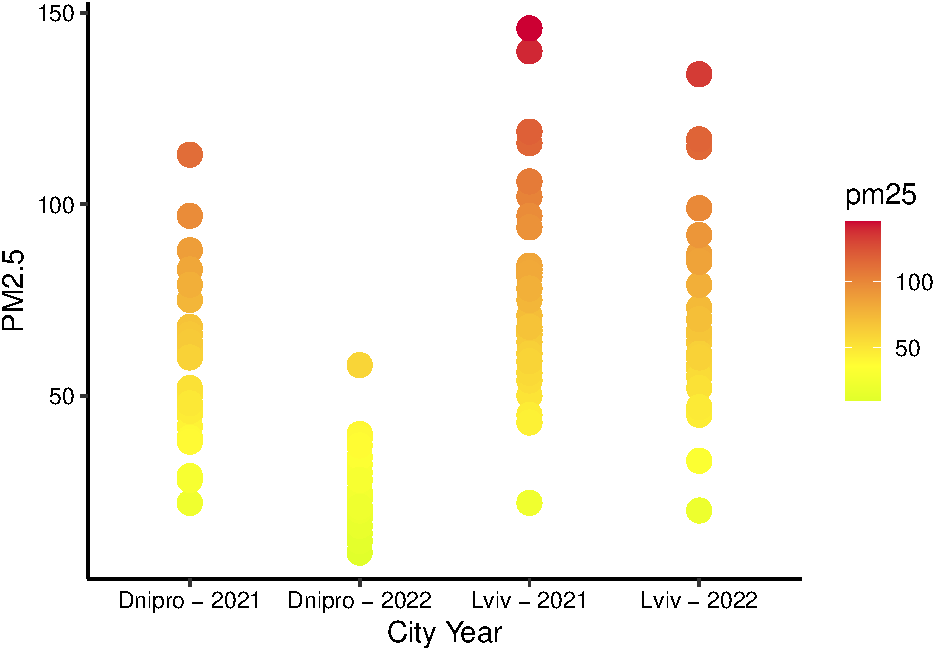
\includegraphics{Fontanie_Gordon_Weinberg_Project_files/figure-latex/plot of pm2.5 air pollution by levels-1.pdf}
\caption{Figure 1 PM2.5 Air Pollution Dot Plot}
\end{figure}

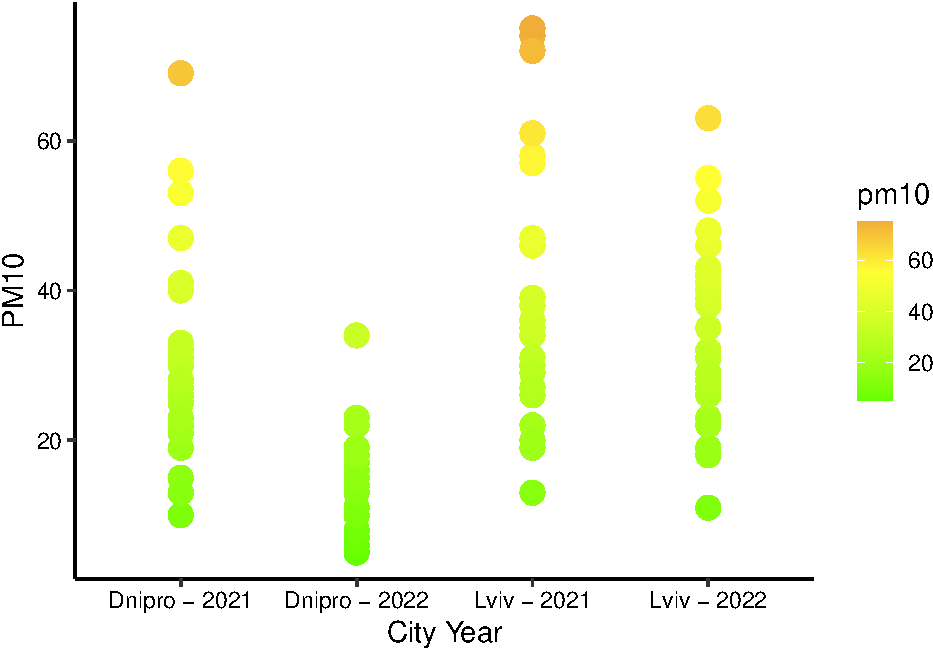
\includegraphics{Fontanie_Gordon_Weinberg_Project_files/figure-latex/plot of pm10 air pollution by levels-1.pdf}
\newpage

\begin{longtable}[]{@{}lrrrr@{}}
\caption{PM2.5 Levels by City}\tabularnewline
\toprule
City & Mean & Min & Max & Std Dev \\
\midrule
\endfirsthead
\toprule
City & Mean & Min & Max & Std Dev \\
\midrule
\endhead
Dnipro & 49.41546 & 4 & 160 & 25.91608 \\
Lviv & 60.51086 & 8 & 518 & 34.79405 \\
\bottomrule
\end{longtable}

\begin{longtable}[]{@{}lrrrr@{}}
\caption{PM10 Levels by City}\tabularnewline
\toprule
City & Mean & Min & Max & Std Dev \\
\midrule
\endfirsthead
\toprule
City & Mean & Min & Max & Std Dev \\
\midrule
\endhead
Dnipro & 24.73309 & 2 & 120 & 15.82186 \\
Lviv & 30.29246 & 4 & 606 & 26.78330 \\
\bottomrule
\end{longtable}

\newpage

\hypertarget{analysis}{%
\section{Analysis}\label{analysis}}

\hypertarget{question-1-are-there-significant-differences-in-air-quality-levels-between-affected-ukrainian-cities-during-the-russian-invasion}{%
\subsection{Question 1: Are there significant differences in air quality
levels between affected Ukrainian cities during the Russian
invasion?}\label{question-1-are-there-significant-differences-in-air-quality-levels-between-affected-ukrainian-cities-during-the-russian-invasion}}

\begin{quote}
{[}Shirley insert text about how we analyzed - visualizations and
statistical tests{]}
\end{quote}

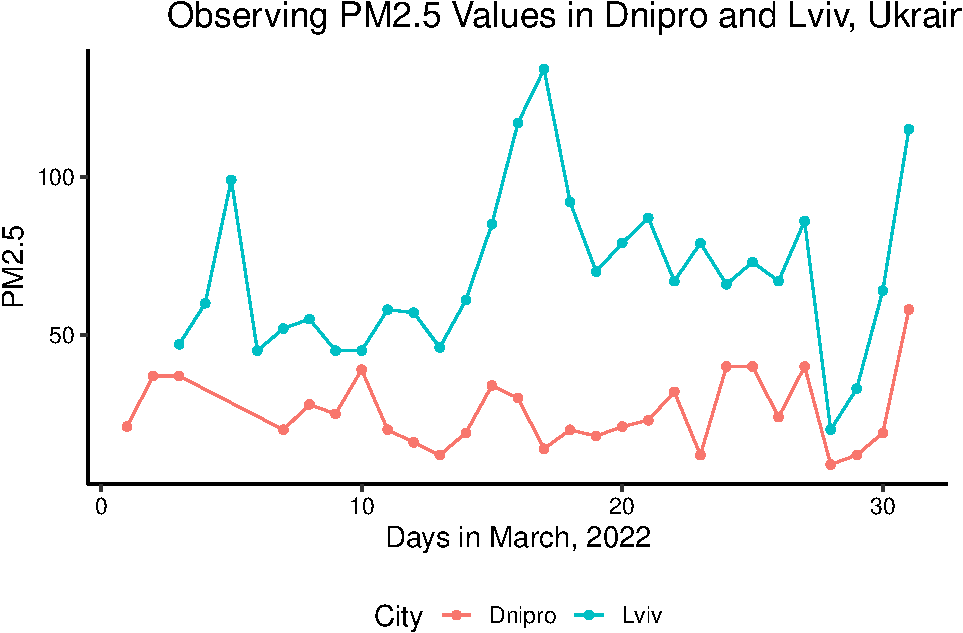
\includegraphics{Fontanie_Gordon_Weinberg_Project_files/figure-latex/Plotting Lviv vs Dnipro-1.pdf}
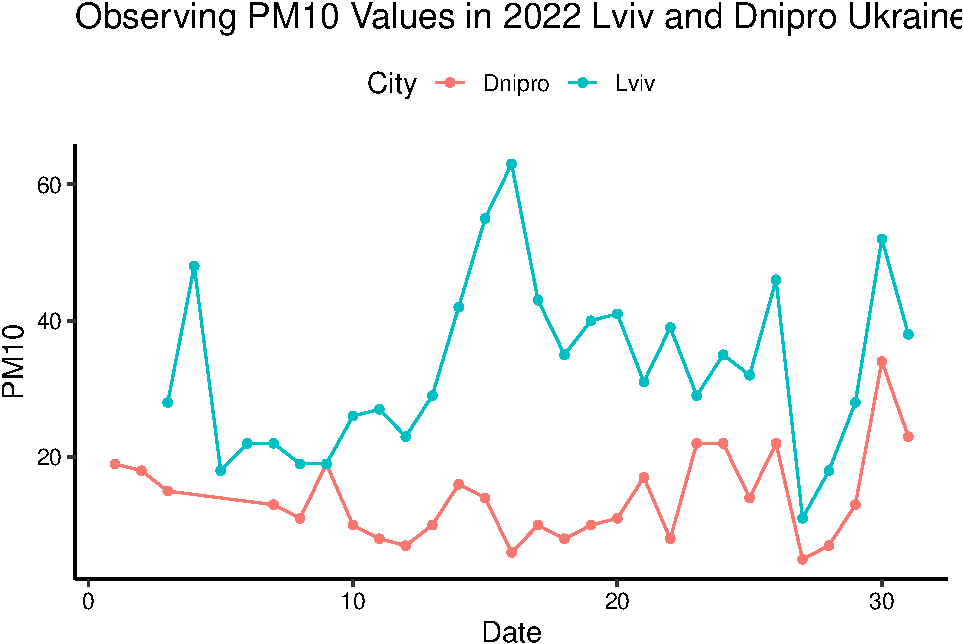
\includegraphics{Fontanie_Gordon_Weinberg_Project_files/figure-latex/Plotting Lviv vs Dnipro-2.pdf}

\begin{verbatim}
## 
## Call:
## lm(formula = pm25 ~ City, data = FULL_Air_quality)
## 
## Residuals:
##     Min      1Q  Median      3Q     Max 
## -49.103 -11.714  -3.103  11.286  64.897 
## 
## Coefficients:
##             Estimate Std. Error t value Pr(>|t|)    
## (Intercept)   25.714      3.791   6.783 8.54e-09 ***
## CityLviv      43.389      5.315   8.164 4.72e-11 ***
## ---
## Signif. codes:  0 '***' 0.001 '**' 0.01 '*' 0.05 '.' 0.1 ' ' 1
## 
## Residual standard error: 20.06 on 55 degrees of freedom
## Multiple R-squared:  0.5479, Adjusted R-squared:  0.5397 
## F-statistic: 66.65 on 1 and 55 DF,  p-value: 4.715e-11
\end{verbatim}

\begin{verbatim}
## 
## Call:
## lm(formula = pm10 ~ City, data = FULL_Air_quality)
## 
## Residuals:
##     Min      1Q  Median      3Q     Max 
## -22.069  -6.000  -1.069   5.931  29.931 
## 
## Coefficients:
##             Estimate Std. Error t value Pr(>|t|)    
## (Intercept)   14.000      1.895   7.388 8.72e-10 ***
## CityLviv      19.069      2.657   7.178 1.93e-09 ***
## ---
## Signif. codes:  0 '***' 0.001 '**' 0.01 '*' 0.05 '.' 0.1 ' ' 1
## 
## Residual standard error: 10.03 on 55 degrees of freedom
## Multiple R-squared:  0.4837, Adjusted R-squared:  0.4743 
## F-statistic: 51.52 on 1 and 55 DF,  p-value: 1.929e-09
\end{verbatim}

\hypertarget{question-2-are-there-significant-differences-in-air-quality-levels-in-affected-ukrainian-cities-before-and-during-the-russian-attacks}{%
\subsection{Question 2: Are there significant differences in air quality
levels in affected Ukrainian cities before and during the Russian
attacks?}\label{question-2-are-there-significant-differences-in-air-quality-levels-in-affected-ukrainian-cities-before-and-during-the-russian-attacks}}

\begin{quote}
Similiar to our first research question, we conducted a visual analysis
of PM2.5 and PM10 levels within Dnipro and Lviv for years 2021 and 2022.
For each of our visualizations, we created line plots that showed the
air pollution levels within the city, comparing 2021 to 2022. As we
needed to visualize the levels of both PM2.5 and PM10, we created four
different plots - ``PM2.5 Levels in Dnipro'', ``PM2.5 Levels in Lviv'',
``PM10 Levels in Dnipro'', and ``PM10 Levels in Lviv''. Within each of
these plots, we also created annotations to indicate the specific dates
of the missile attacks within the cities to see if there were any PM2.5
or PM10 increases or decreases around those dates. Additionally, we
conducted a linear regression analysis for each of these charts to
understand if there is a significant difference in PM2.5 levels and PM10
levels within Dnipro and Lviv in March of 2021 compared to March of
2022.\\
\end{quote}

\newpage

\begin{quote}
\textbf{PM2.5 in Dnipro}\\
When plotting PM2.5 levels in Dnipro in 2021 compared to 2022, it is
evident that overall, PM2.5 levels were higher in 2021 than 2022. It is
also interesting to note that around March 11 in 2022, when the missile
attack occured, there appears to be an uptick in PM2.5 levels and then
sharply decreases shortly after. Overall in both years, there seems to
be a variety of fluctuation in PM2.5 levels and they are not consistent
within each year. Additionally, within most of 2022, PM2.5 levels stayed
within ``good'' to ``moderate'' levels, with an exception of reaching a
level of ``unhealthy for sensitive groups'' at the end of March 2022. In
March 2021, however, the PM2.5 levels were mainly in the ``unhealthy for
sensitive groups'' or ``unhealthy'' category, with only a few days
throughout that month in ``moderate'' levels.
\end{quote}

\begin{quote}
For the statistical analysis, we ran a linear regression model of pm2.5
levels by year within Dnipro, to understand if there are significant
differences in PM2.5 levels within the city in March 2021 compared to
March 2022. The linear regression showed the slope was negative
(-32.253), meaning that PM2.5 levels decreased in 2022 compared to 2021.
Additionally, the linear regression showed that the relationship between
PM2.5 levels and year in Dnipro is significant (p = 5.074e-10), meaning
that there is a significant difference in PM2.5 levels in Dnipro in 2022
compared to 2021.
\end{quote}

\begin{figure}
\centering
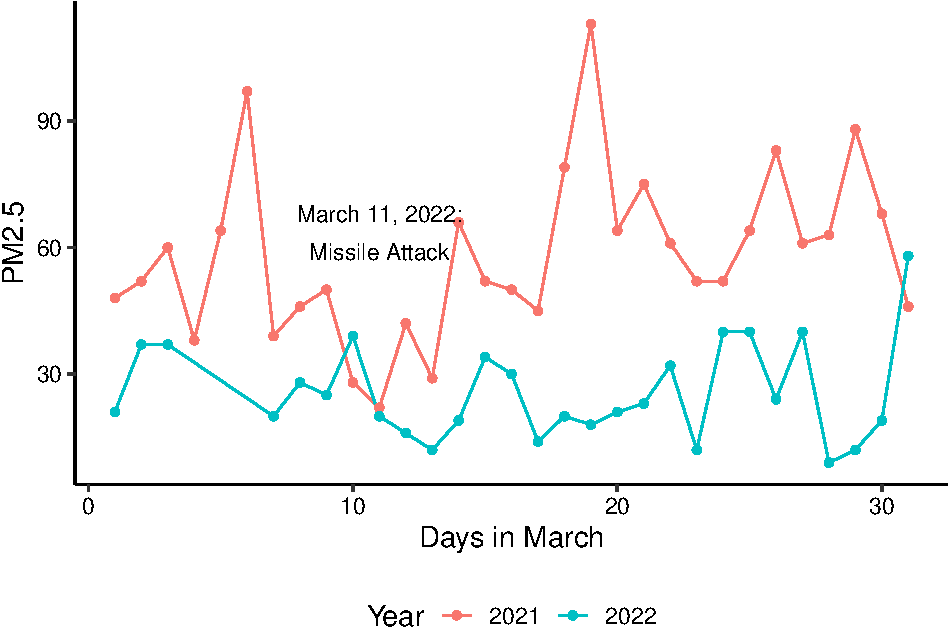
\includegraphics{Fontanie_Gordon_Weinberg_Project_files/figure-latex/Visualizing PM25 in Dnipro-1.pdf}
\caption{PM2.5 Levels in Dnipro}
\end{figure}

\newpage

\begin{quote}
\textbf{PM2.5 in Lviv}\\
When plotting PM2.5 levels in Lviv in 2021 compared to 2022, there is no
clear difference in levels between years. It is interesting to note that
before the March 18 attack, PM2.5 levels were increasing, and after the
March 18, 2022 missile attack, it appears levels sharply decreased.
Overall in both years, it appears that there seems to be a variety of
fluctuation in PM2.5 in Lviv. Additionally, within both 2021 and 2022,
it is very rare that levels are within the ``good'' range of PM2.5
(\textless15.4) and are typically within ``moderate'' to ``unhealthy''
levels.
\end{quote}

\begin{quote}
For the statistical analysis, we ran a linear regression model of PM2.5
levels by year within Lviv, to understand if there are significant
differences in levels within the city in March 2021 compared to March
2022. Through the analysis, we found that the slope was negative
(-10.284), meaning that PM2.5 levels decreased in 2022 compared to 2021.
However, the linear regression showed that the negative relationship
between PM2.5 levels and year in Lviv is not significant (p=0.1639).
\end{quote}

\begin{figure}
\centering
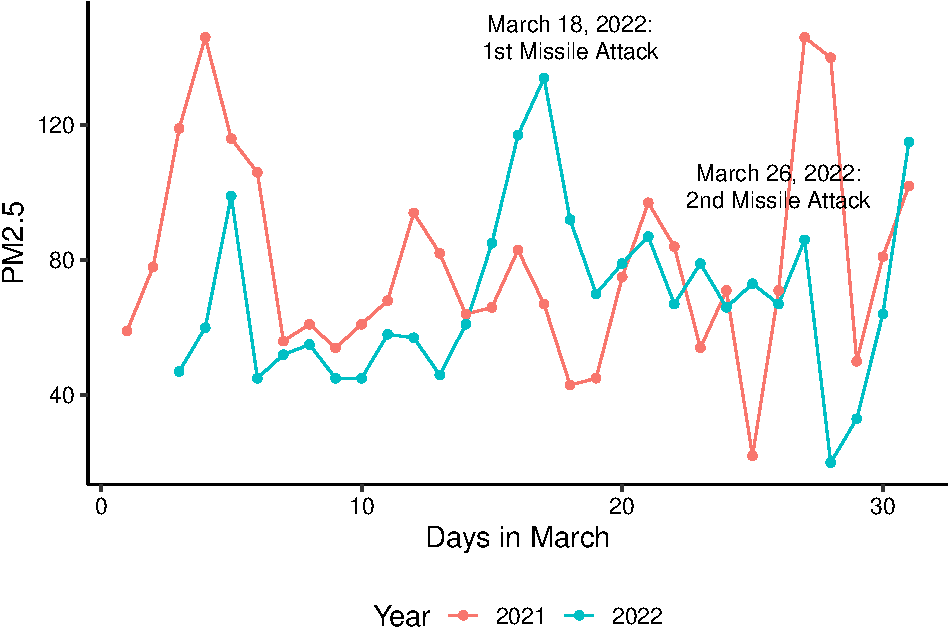
\includegraphics{Fontanie_Gordon_Weinberg_Project_files/figure-latex/visualizing PM25 in Lviv-1.pdf}
\caption{PM2.5 Levels in Lviv}
\end{figure}

\newpage

\begin{quote}
\textbf{PM10 in Dnipro}\\
When plotting PM10 levels in Dnipro in 2021 compared to 2022, it is
evident that overall, PM10 levels were higher in 2021 compared to 2022.
When looking at the PM10 levels around the March 11 attack in 2022,
there does not appear to be a significant increase. Additionally, in
March 2022, PM10 levels seemed to stay within or below ``moderate''
levels, whereas 2021 levels ranged from ``moderate'' to ``unhealthy for
sensitive groups''.
\end{quote}

\begin{quote}
For the statistical analysis, we ran a linear regression of PM10 levels
by year within Dnipro, to understand if there are significant
differences in levels within the city in March 2021 compared to March
2022. Through the analysis, we found that the slope was negative
(-15.677), meaning that PM10 levels decreased in 2022 compared to 2021.
Additionally, the linear regression showed that these results are
statistically significant (p=4.325e-07), meaning there is a significant
difference in PM10 levels in Dnipro in 2022 compared to 2021.
\end{quote}

\begin{figure}
\centering
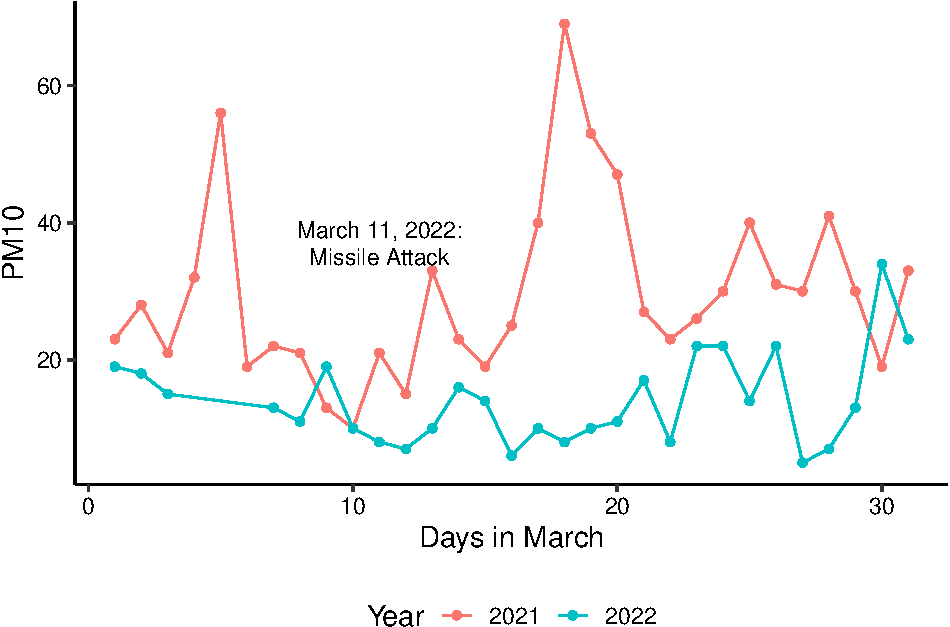
\includegraphics{Fontanie_Gordon_Weinberg_Project_files/figure-latex/visualizing PM10 in Dnipro-1.pdf}
\caption{PM10 Levels in Dnipro}
\end{figure}

\newpage

\begin{quote}
\textbf{PM10 in Lviv}\\
When plotting PM10 levels in Lviv in 2021 compared to 2022, there is no
clear difference observed in PM10 levels between the years. It is also
interesting to note that there does not seem to a significant change in
PM10 levels after the March 18 attack, and PM10 levels appear to sharply
drop after the March 26 attack. Additionally, PM10 levels in both years
stay mainly within ``unhealthy for sensitive groups'' to ``good''
levels, but at some points in 2021, levels reach into the ``unhealthy''
level.
\end{quote}

\begin{quote}
For the statistical analysis, we ran a linear regression of PM10 levels
by year within Lviv, to understand if there are significant differences
in levels within the city in March 2021 compared to March 2022. Through
the analysis, we found that the slope was negative (-5.673), meaning
that PM10 levels decreased in 2022 compared to 2021 in Lviv. However,
the linear regression showed that these results are not statistically
significant (p=0.1364), meaning that there is not a significant
difference in PM10 levels in Lviv in 2022 compared to 2021.
\end{quote}

\begin{figure}
\centering
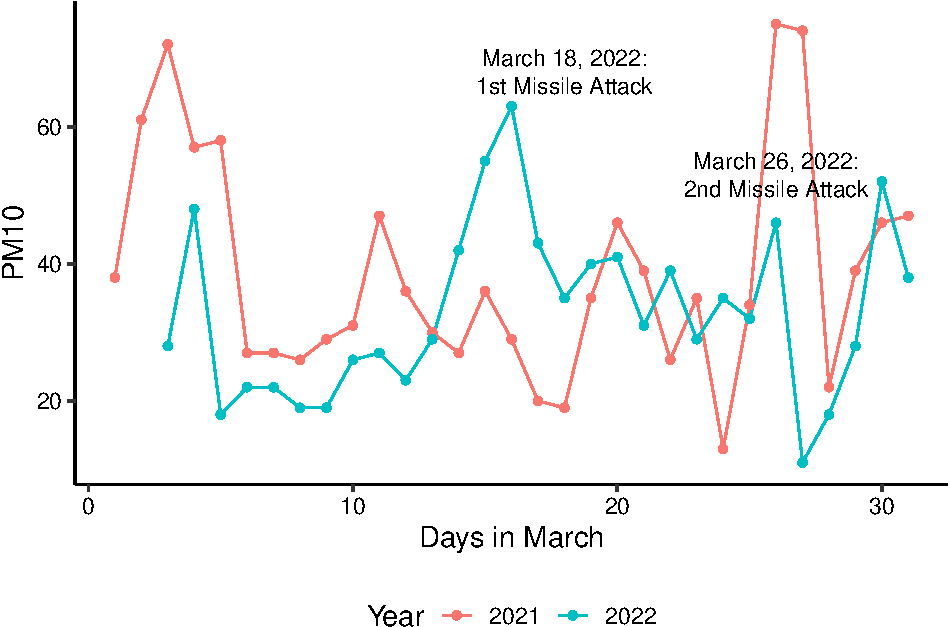
\includegraphics{Fontanie_Gordon_Weinberg_Project_files/figure-latex/visualizing PM10 in Lviv-1.pdf}
\caption{PM10 Levels in Lviv}
\end{figure}

\newpage

\hypertarget{summary-and-conclusions}{%
\section{Summary and Conclusions}\label{summary-and-conclusions}}

\hypertarget{question-1-are-there-significant-differences-in-air-quality-levels-between-affected-ukrainian-cities-during-the-russian-invasion-1}{%
\subsection{Question 1: Are there significant differences in air quality
levels between affected Ukrainian cities during the Russian
invasion?}\label{question-1-are-there-significant-differences-in-air-quality-levels-between-affected-ukrainian-cities-during-the-russian-invasion-1}}

\begin{quote}
{[}insert results from our analysis{]}
\end{quote}

\hypertarget{question-2-are-there-significant-differences-in-air-quality-levels-in-affected-ukrainian-cities-before-and-during-the-russian-attacks-1}{%
\subsection{Question 2: Are there significant differences in air quality
levels in affected Ukrainian cities before and during the Russian
attacks?}\label{question-2-are-there-significant-differences-in-air-quality-levels-in-affected-ukrainian-cities-before-and-during-the-russian-attacks-1}}

\begin{quote}
{[}insert text about summary{]}
\end{quote}

\begin{quote}
insert text about what may have affected our results, limitations of our
data, and what we would do next if we could
\end{quote}

\newpage

\hypertarget{references}{%
\section{References}\label{references}}

\textless add references here if relevant, otherwise delete this
section\textgreater{}

\end{document}
